\documentclass[tikz,border=2pt]{standalone}
\usepackage{amsmath,amssymb}
\usepackage{tikz}
\usetikzlibrary{arrows.meta}

\begin{document}
% The simplex path on the Giapetto polygon: start at the origin and move along edges to an
% adjacent corner with a better objective value until none is better.
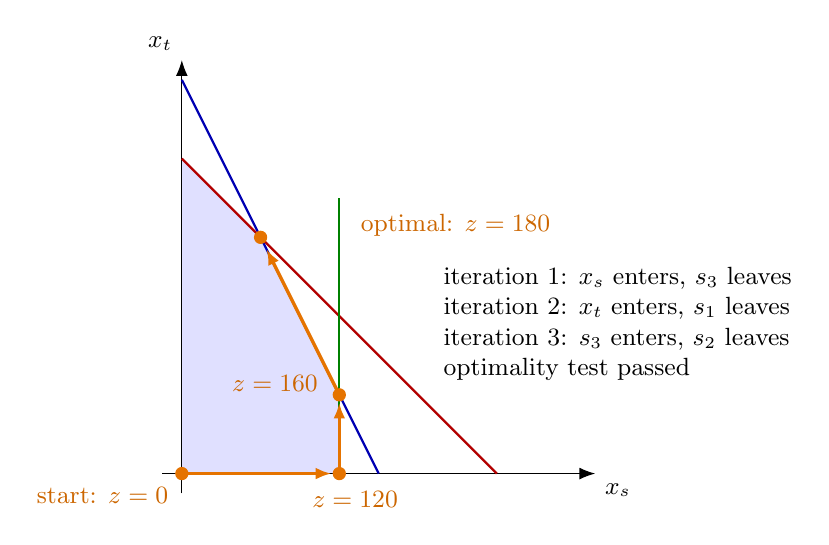
\begin{tikzpicture}[x=0.05cm, y=0.05cm, every node/.style={font=\small}, >={Latex[length=2mm]}]
	\fill[blue!12] (0,0) -- (40,0) -- (40,20) -- (20,60) -- (0,80) -- cycle;
	\draw[->] (-5,0) -- (105,0) node[below right] {$x_s$};
	\draw[->] (0,-5) -- (0,105) node[above left] {$x_t$};
	\draw[blue!70!black, thick] (50,0) -- (0,100);
	\draw[red!70!black, thick] (80,0) -- (0,80);
	\draw[green!50!black, thick] (40,0) -- (40,70);
	\draw[->, orange!90!black, very thick] (0,0) -- (38,0);
	\draw[->, orange!90!black, very thick] (40,0) -- (40,18);
	\draw[->, orange!90!black, very thick] (40,20) -- (21.5,57);
	\foreach \p in {(0,0),(40,0),(40,20),(20,60)} {\fill[orange!90!black] \p circle (2.4pt);}
	\node[orange!80!black, font=\small, anchor=north east] at (-1,-1) {start: $z=0$};
	\node[orange!80!black, font=\small, anchor=north] at (44,-2) {$z=120$};
	\node[orange!80!black, font=\small, anchor=east] at (37,23) {$z=160$};
	\node[orange!80!black, font=\small, anchor=west] at (43,63) {optimal: $z=180$};
	\node[font=\small, anchor=west, align=left] at (64,38) {iteration 1: $x_s$ enters, $s_3$ leaves\\ iteration 2: $x_t$ enters, $s_1$ leaves\\ iteration 3: $s_3$ enters, $s_2$ leaves\\ optimality test passed};
	\end{tikzpicture}
\end{document}
